\indent LDM was based on the U-Net3D architecture.
\subparagraph{Configuration}\mbox{}\\

\begin{table}[H]
\centering
\begin{tabular}{|l|l|}
\hline
\textbf{Parameter} & \textbf{Value} \\
\hline
\multicolumn{2}{|c|}{\textbf{Training}} \\
\hline
Batch Size & 5 \\
\hline
Seed & 42 \\
\hline
Epochs & 15000 \\
\hline
Training Ratio & 0.9 \\
\hline
Number of Nodes & 1 \\
\hline
Number of Devices & 1 \\
\hline
Device & CUDA \\
\hline
Float precision & 32 \\
\hline
Metric to Monitor & val/loss \\
\hline
Metric Mode & Min \\
\hline
\multicolumn{2}{|c|}{\textbf{Model}} \\
\hline
Learning Rate & 0.0001 \\
\hline
Loss Type & L1 \\
\hline
VQGAN Checkpoint Path & \url{./models/meta_vqgan/checkpoints/meta_vqgan-v5.ckpt} \\
\hline
Probability of Focus Present & 0.0 \\
\hline
Gradient Scaler Enabled & False \\
\hline
Focus Present Mask & Null \\
\hline
Max Gradient Norm & Null \\
\hline
\multicolumn{2}{|c|}{\textbf{EMA Configuration}} \\
\hline
Decay & 0.995 \\
\hline
Start Step & 2000 \\
\hline
Update Every Step & 10 \\
\hline
\multicolumn{2}{|c|}{\textbf{Hidden Scan Representation}} \\
\hline
Image Size & 64 \\
\hline
Depth Size & 16 \\
\hline
Number of Channels & 8 \\
\hline
\multicolumn{2}{|c|}{\textbf{Scheduler Parameters}} \\
\hline
Timesteps & 300 \\
\hline
\multicolumn{2}{|c|}{\textbf{UNet Parameters}} \\
\hline
Dimension Multipliers & [1, 2, 4, 8] \\
\hline
\multicolumn{2}{|c|}{\textbf{Dataset Configuration}} \\
\hline
Caching & Disk \\
\hline
Path & \url{/ravana/d3d_work/micorl/data/ct_images_prostate_32fixed/} \\
\hline
Image Size & 128 \\
\hline
Number of Slices & 32 \\
\hline
Window Width & 400 \\
\hline
Window Level & 60 \\
\hline
\end{tabular}
\caption{Configuration of the Medical Diffusion LDM.}
\label{table:meta_diffuser_params}
\end{table}

\subparagraph{Training}\mbox{}\\

\indent Throughout the first 2000 epochs, losses consistently decreased in both the training and validation phases but after they stood still. Nevertheless, it was decided to continue the training until the end - epoch 15000.
\begin{figure}[H]
\minipage{0.49\textwidth}
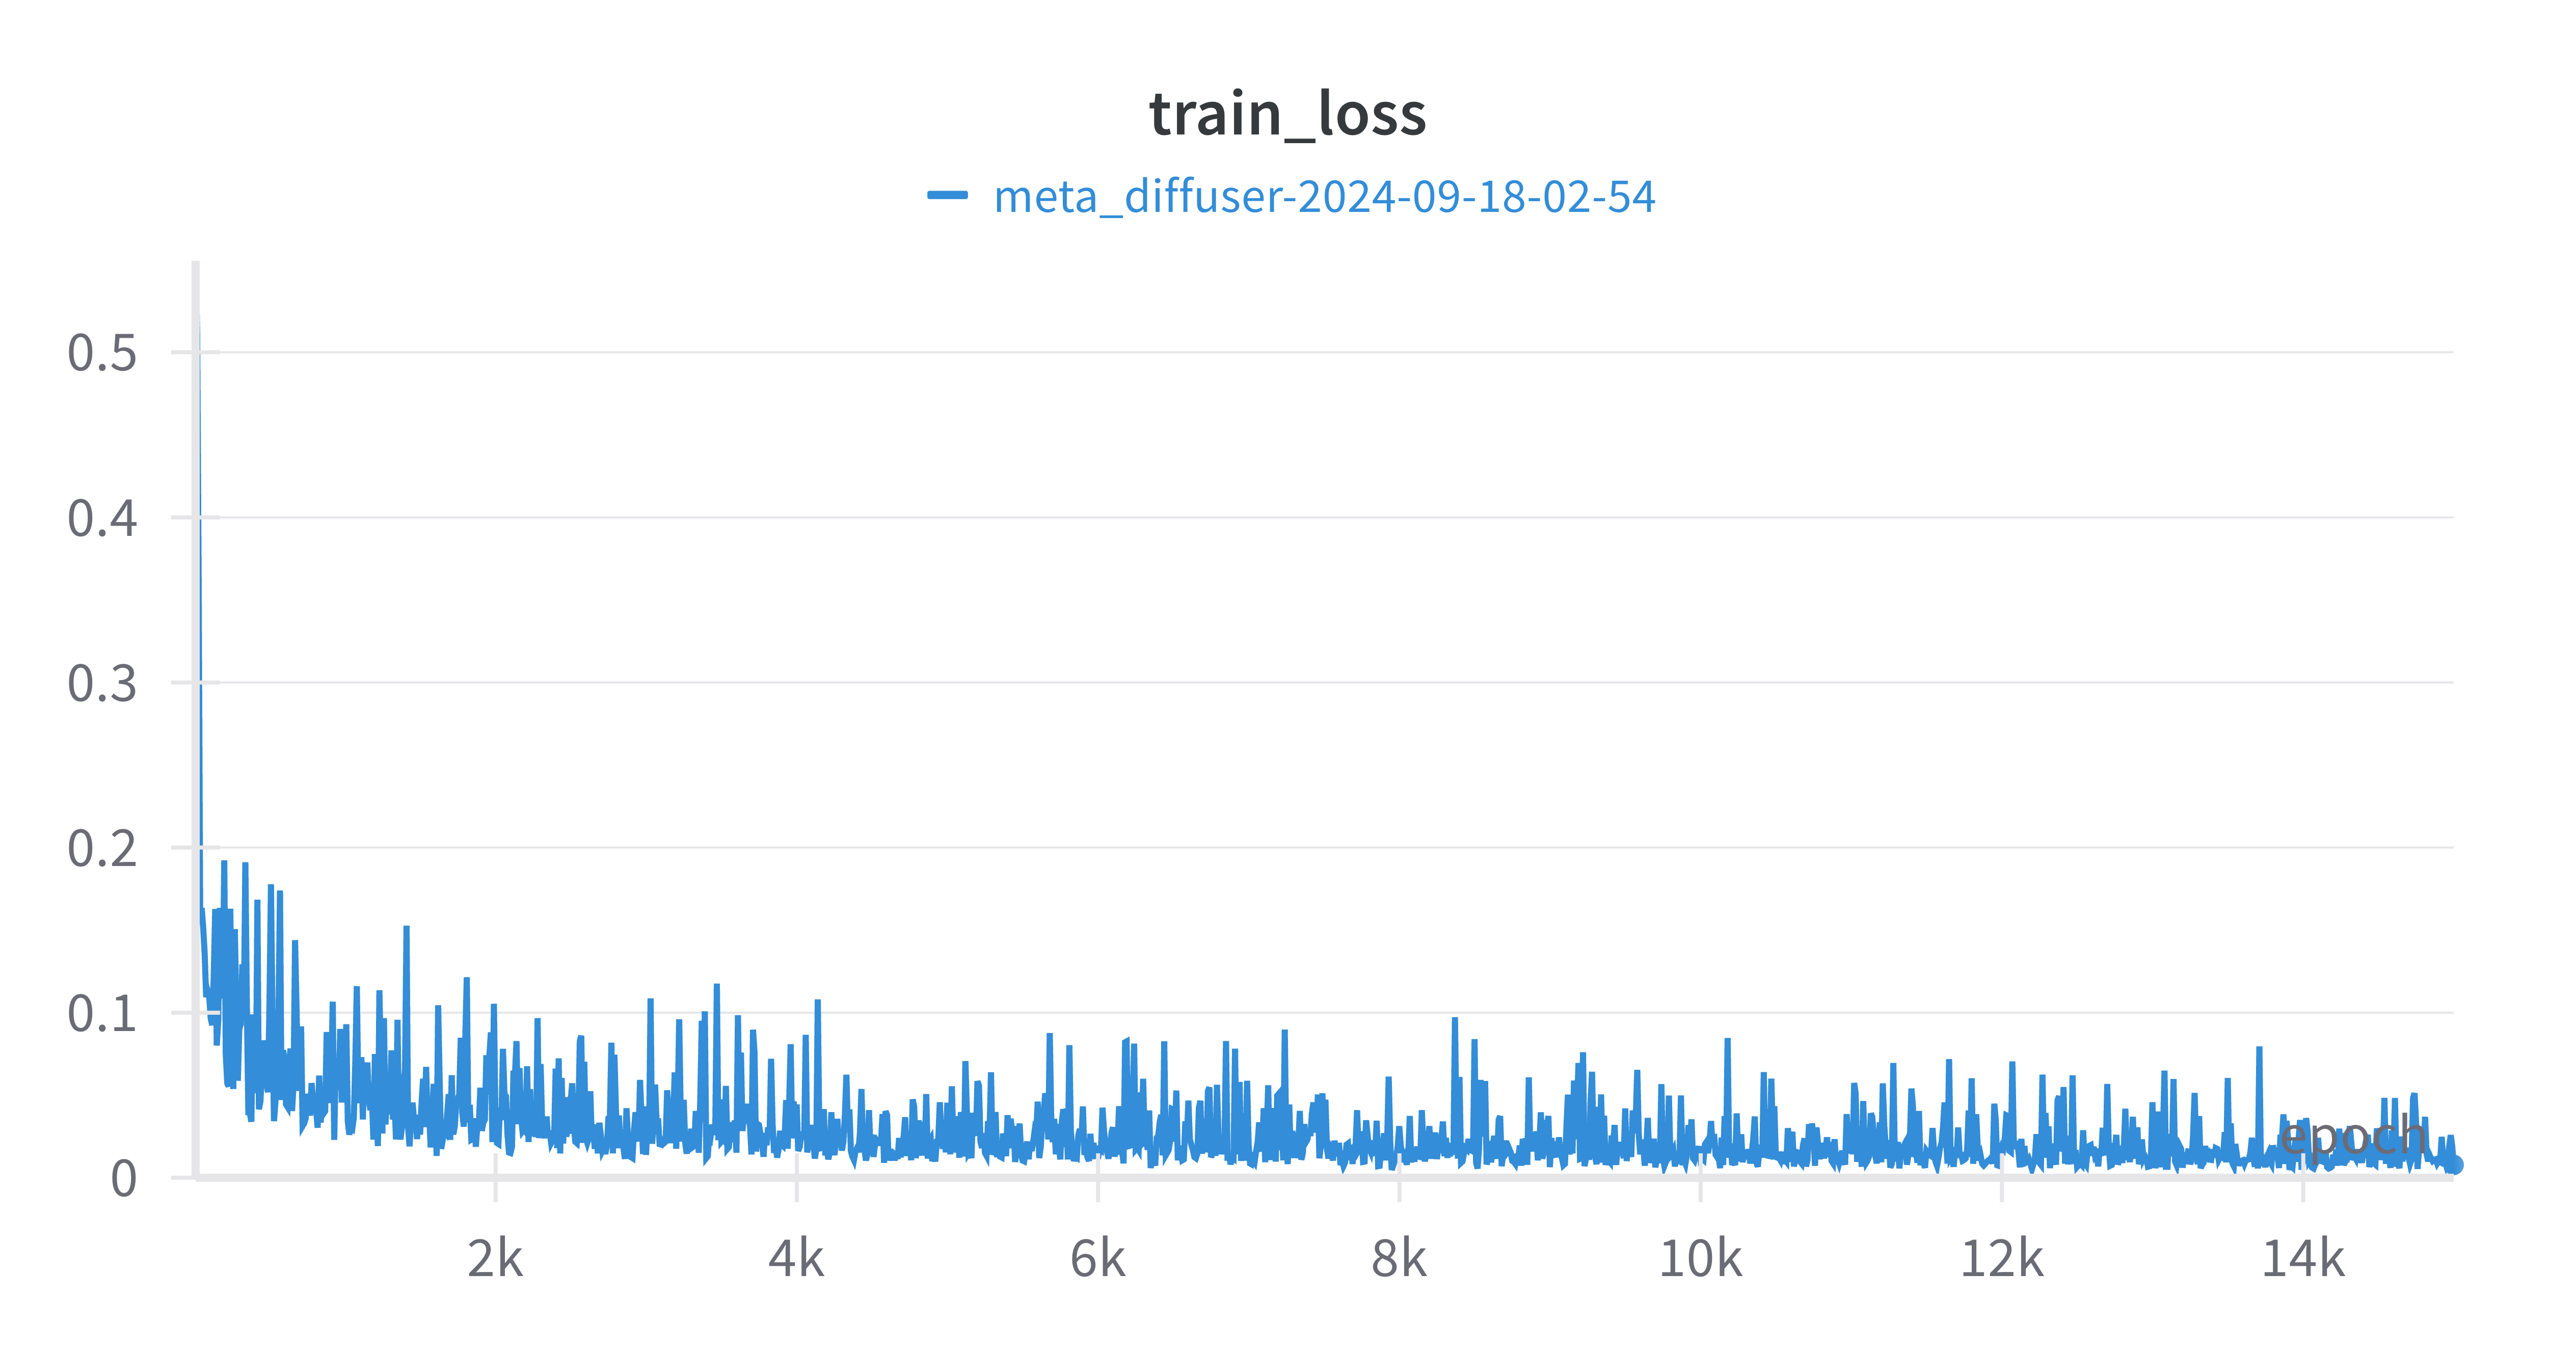
\includegraphics[width=\linewidth]{detailed_engineering/Meta Diffusion/charts/train_loss.png}
\caption{Loss during the training. Lower is better.}
\endminipage\hfill
\minipage{0.49\textwidth}
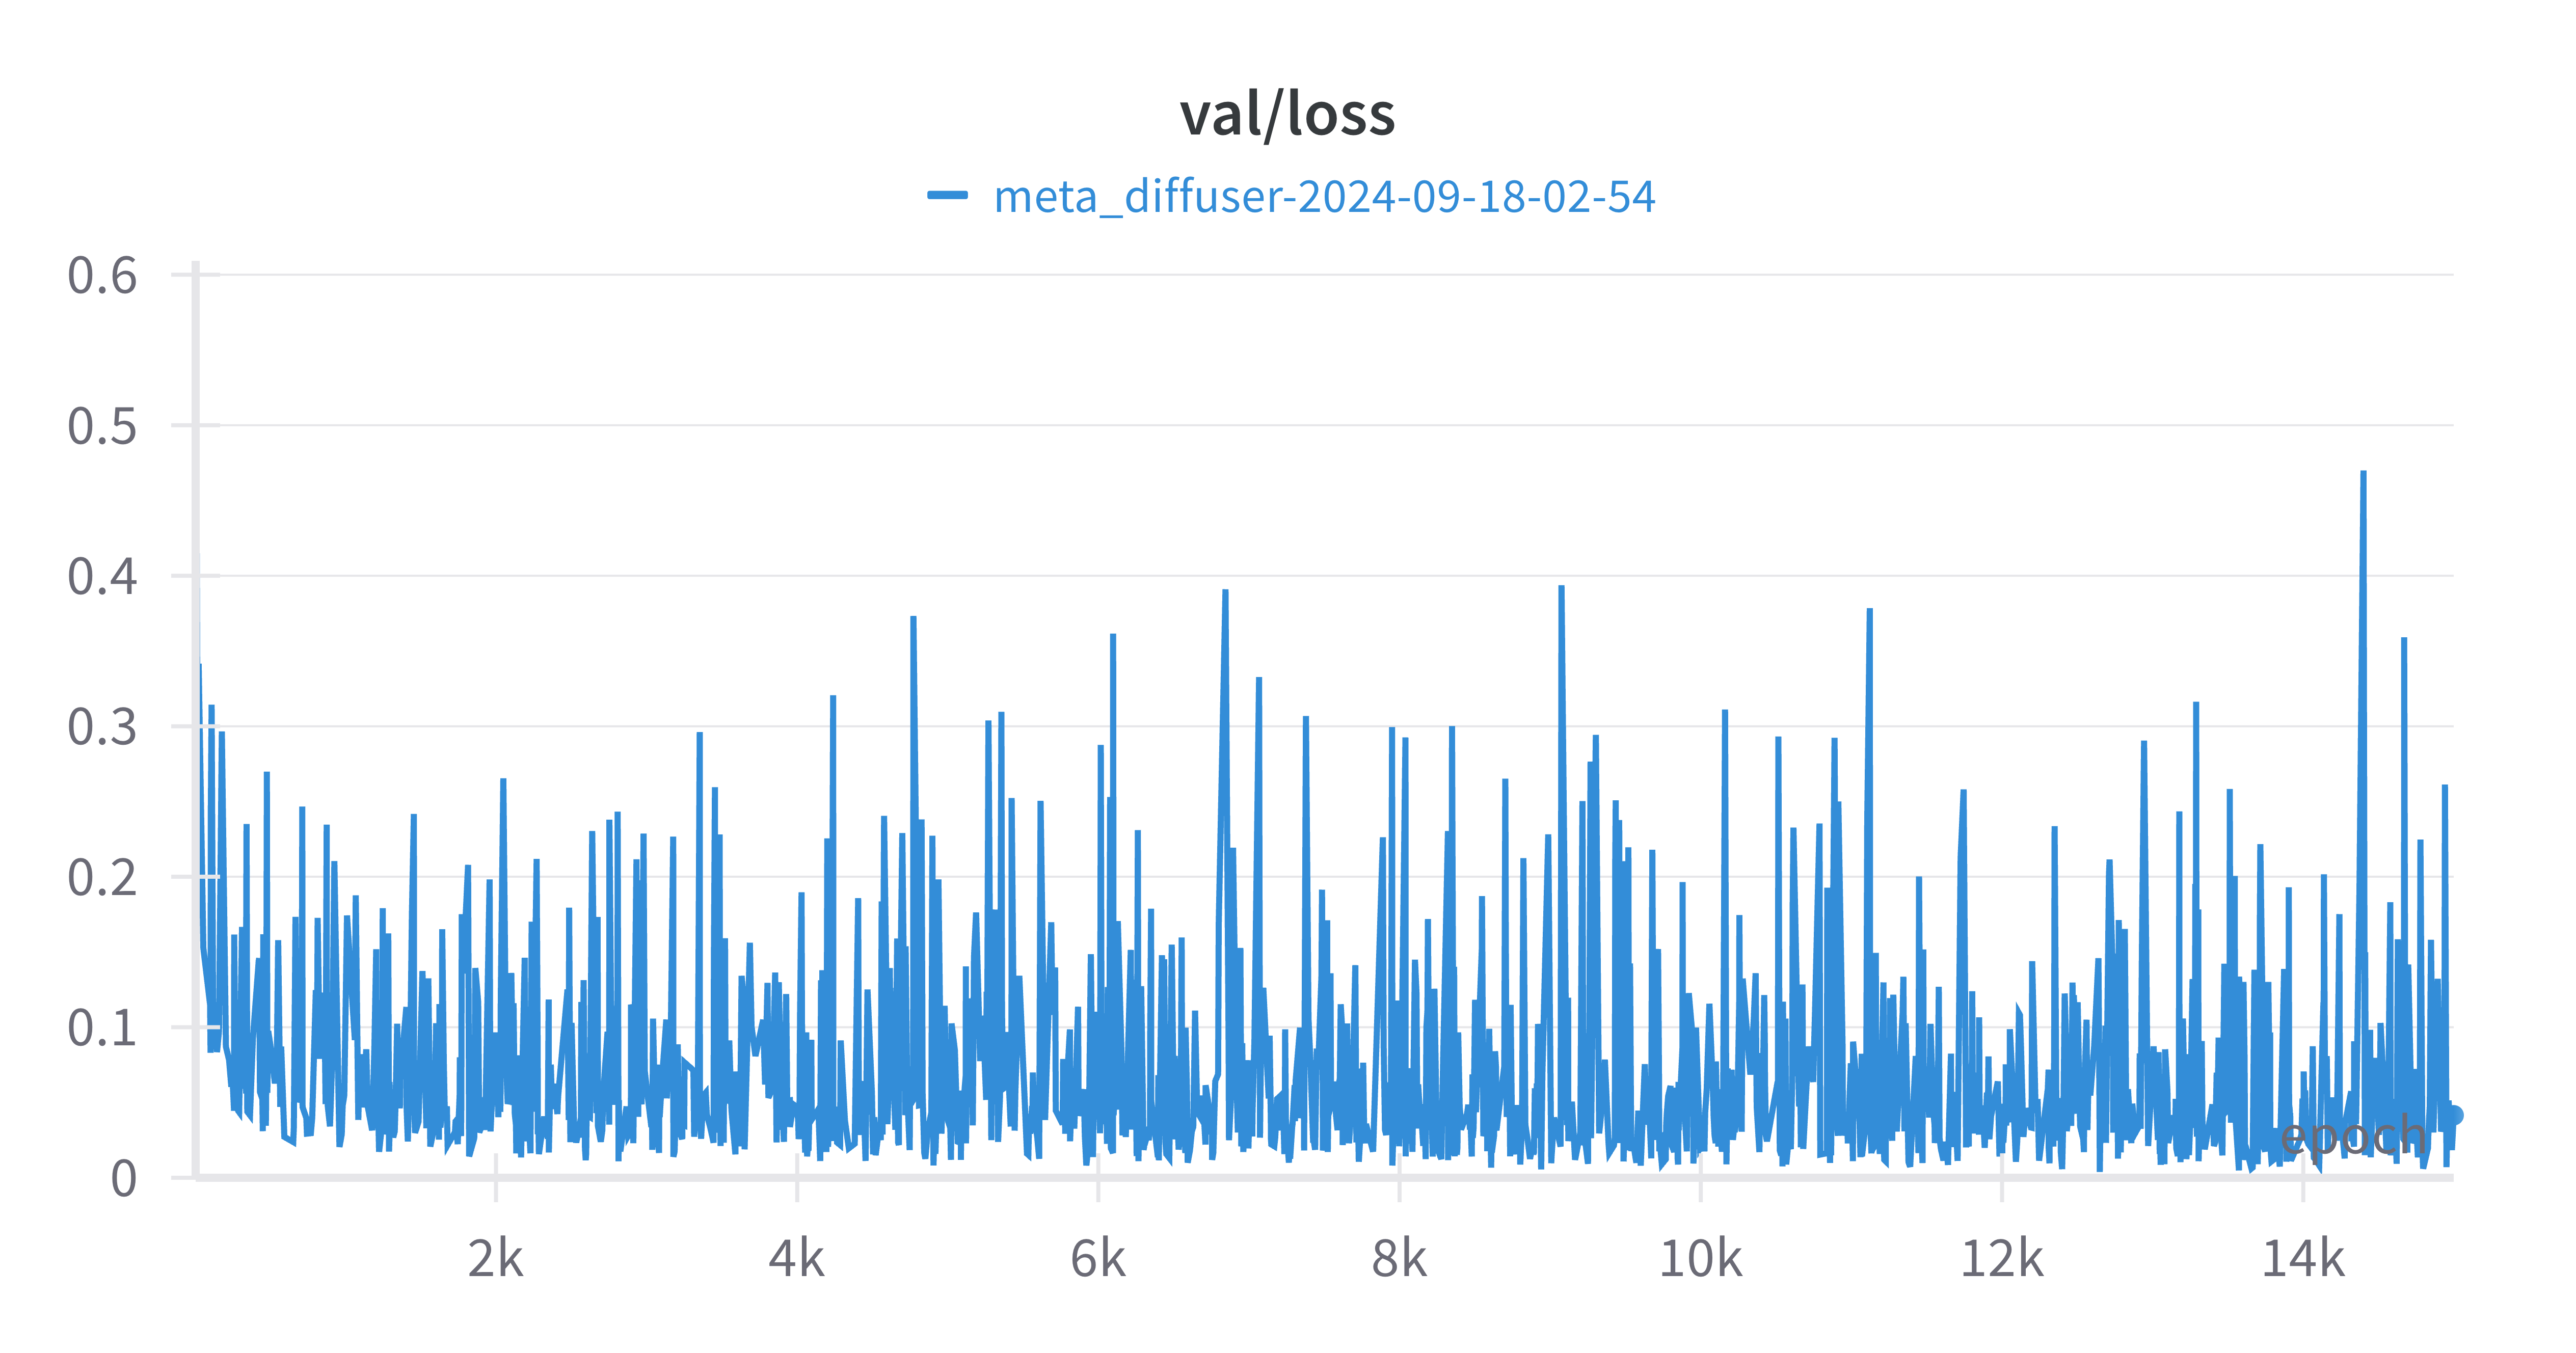
\includegraphics[width=\linewidth]{detailed_engineering/Meta Diffusion/charts/val_loss.png}
\caption{Loss during the validation. Lower is better.}
\endminipage
\end{figure}

Additional metrics evaluating the quality of the generated scan.
\begin{figure}[H]
\minipage{0.49\textwidth}
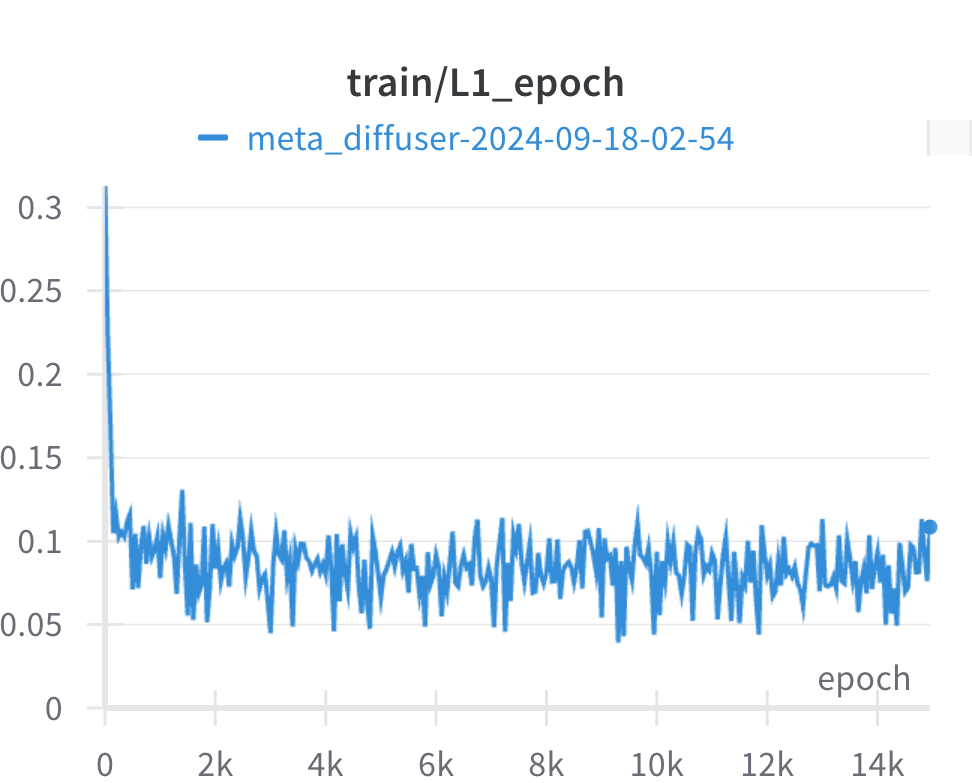
\includegraphics[width=\linewidth]{detailed_engineering/Meta Diffusion/charts/train_l1_epoch.png}

\endminipage\hfill
\minipage{0.49\textwidth}
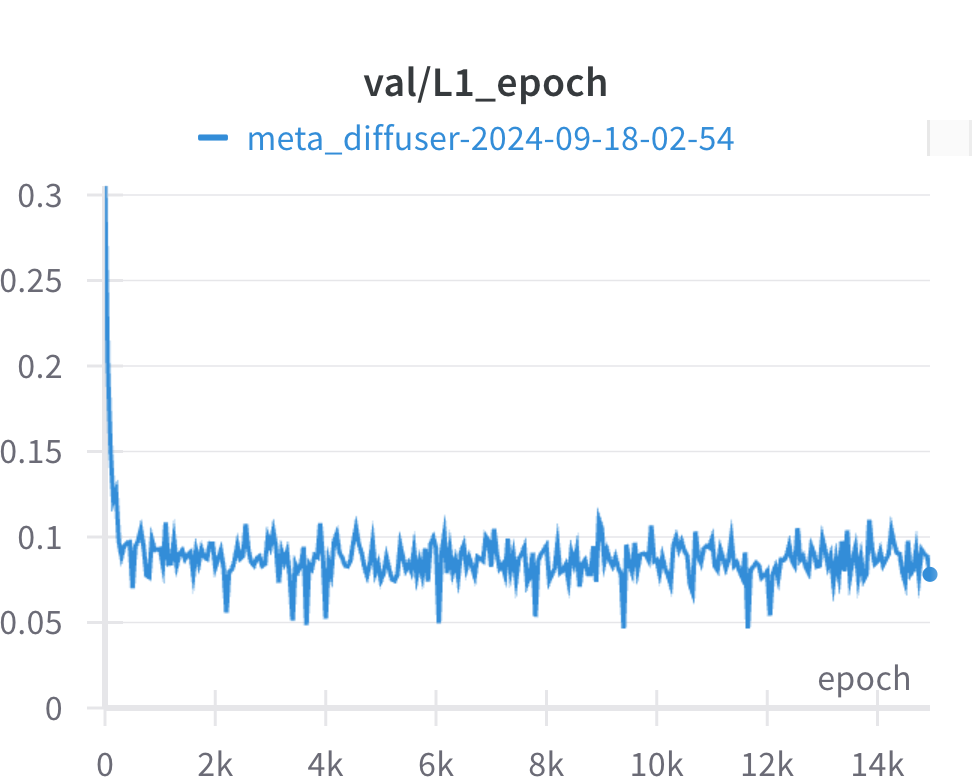
\includegraphics[width=\linewidth]{detailed_engineering/Meta Diffusion/charts/val_l1_epoch.png}

\endminipage
\caption{L1 between two generated CT scans and two random samples from the training/validation datasets. Lower is better.}
\end{figure}

\begin{figure}[H]
\minipage{0.49\textwidth}
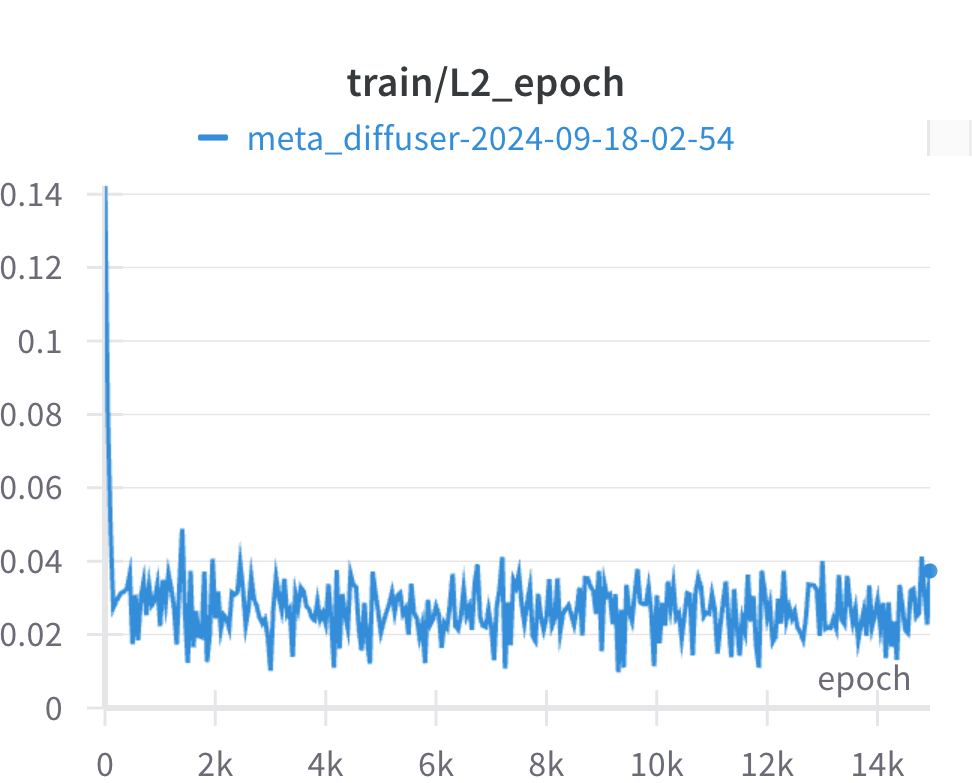
\includegraphics[width=\linewidth]{detailed_engineering/Meta Diffusion/charts/train_l2_epoch.png}

\endminipage\hfill
\minipage{0.49\textwidth}
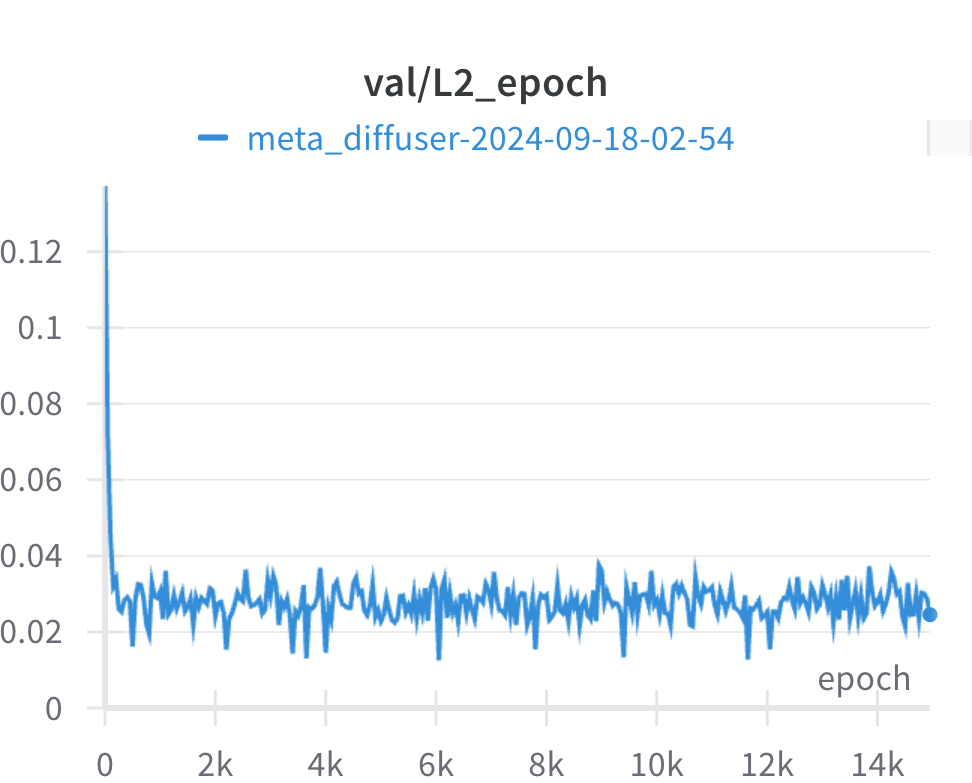
\includegraphics[width=\linewidth]{detailed_engineering/Meta Diffusion/charts/val_l2_epoch.png}

\endminipage
\caption{L2 between two generated CT scans and two random samples from the training/validation datasets. Lower is better.}
\end{figure}

\begin{figure}[H]
\minipage{0.49\textwidth}
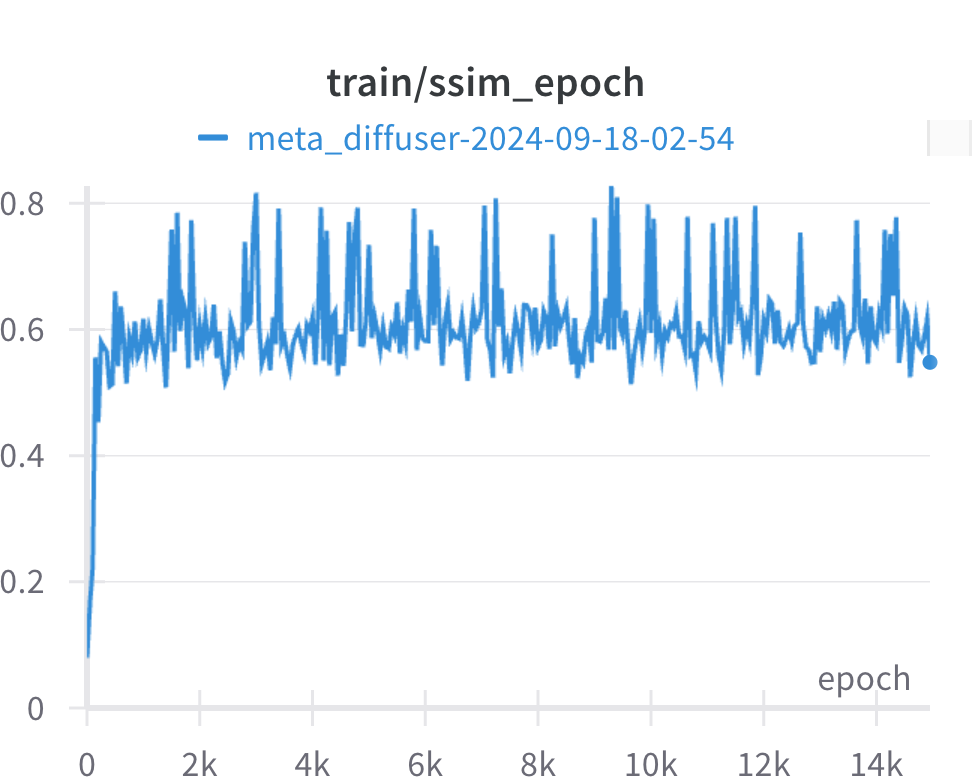
\includegraphics[width=\linewidth]{detailed_engineering/Meta Diffusion/charts/train_ssim_epoch.png}

\endminipage\hfill
\minipage{0.49\textwidth}
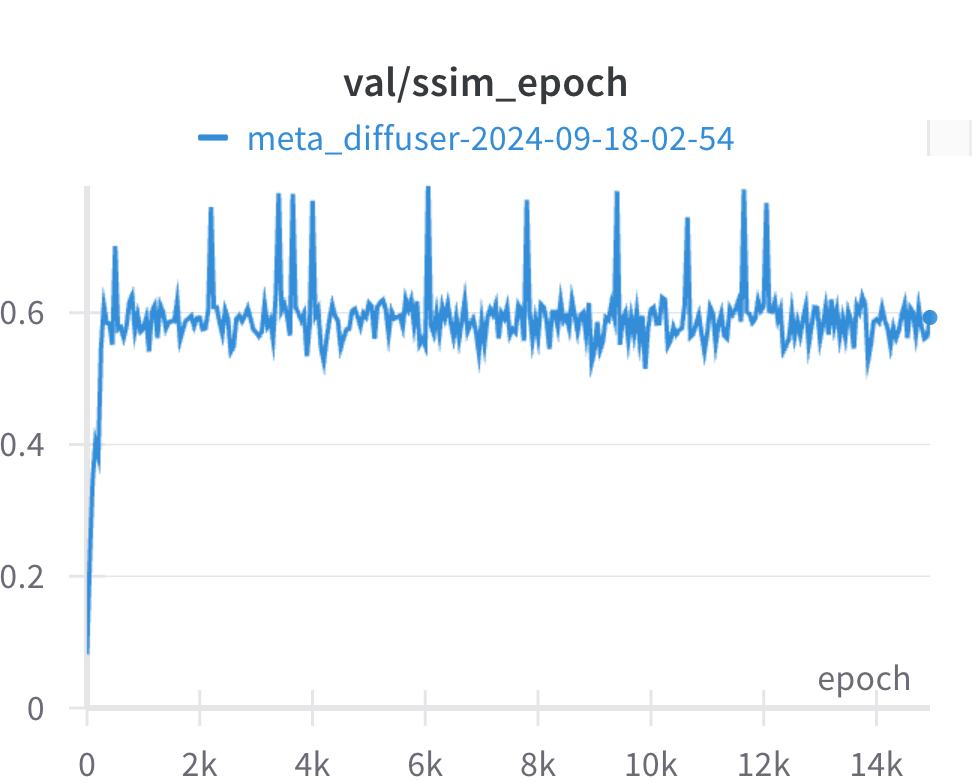
\includegraphics[width=\linewidth]{detailed_engineering/Meta Diffusion/charts/val_ssim_epoch.png}

\endminipage
\caption{SSIM between two generated CT scans and two random samples from the training/validation datasets. Higher is better.}
\end{figure}

\subparagraph{Results}\mbox{}\\
\indent The resulting exemplary scan of the figure \ref{fig:random_ldm} produced by the latent diffusion model is visually coherent and looks real to the amateur. The comparison between one sample of the input data set and the generated scan in the figure \ref{fig:ldm-success-comparison} shows that there is not much difference between them. The model is a good candidate for the evaluation phase.

% \begin{figure}[H]
%     \centering
%     \includegraphics[width=\linewidth]{}
%     \caption{Caption}
%     \label{fig:enter-label}
% \end{figure}
\begin{figure}[H]
    \centering
    % \includegraphics{}
     \animategraphics[width=0.6\textwidth, loop, autoplay]{5}%frame rate
    {detailed_engineering/Meta Diffusion/generation/layer-}%path to figures
    {0}%start index
    {31}%end index
    \caption{Random layer of a synthetic CT scan generated from Gaussian noise.}
    \label{fig:random_ldm}
\end{figure}

\begin{figure}[H]
    \centering
    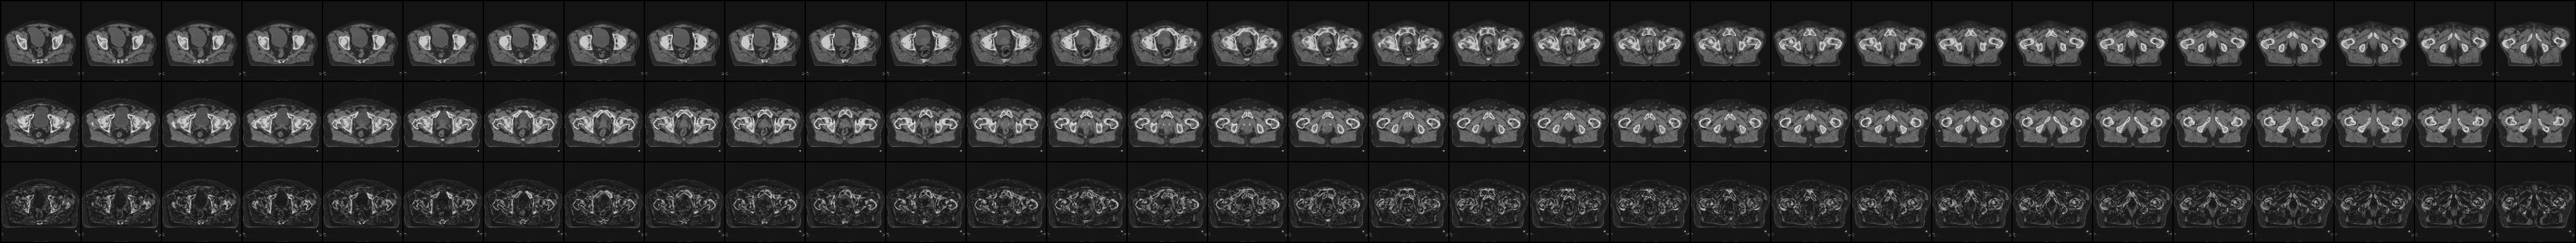
\includegraphics[width=\linewidth]{detailed_engineering/Meta Diffusion/charts/meta_diffusion_comparison.png}
    \caption{Top - first sample from training dataset, middle - synthetic CT scan, bottom - L1 difference between them.}
    \label{fig:ldm-success-comparison}
\end{figure}